\documentclass{bioinfo}
\copyrightyear{2020} \pubyear{2020}

\access{Advance Access Publication Date: Day Month Year}
\appnotes{Manuscript Category}

\begin{document}
\firstpage{1}

\subtitle{Application Notes}

\title[short Title]{jax-unirep: An accelerated, performant, and user-friendly implementation of UniRep using JAX}
\author[Sample \textit{et~al}.]{
    Arkadij Kummer\,$^{\text{\sfb 1}*}$, Ivan Jayapurna\,$^{\text{\sfb 2,}}$ and Eric J. Ma\,$^{\text{\sfb 3,}*}$}
\address{
    $^{\text{\sf 1}}$Global Discovery Chemistry, Novartis Institutes for Biomedical Research, Basel, Switzerland \\
    $^{\text{\sf 2}}$University of California at Berkeley, Berkeley, CA, United States of America \\
    $^{\text{\sf 3}}$NIBR Informatics, Novartis Institutes for Biomedical Research, Cambridge, MA, United States of America \\
}

\corresp{$^\ast$To whom correspondence should be addressed.}

\history{Received on XXXXX; revised on XXXXX; accepted on XXXXX}

\editor{Associate Editor: XXXXXXX}

\abstract{
    \textbf{Summary:} We provide an upgraded version of UniRep,
    a recurrent neural network model trained on 24 million protein sequences,
    with significant speed improvements,
    API enhancements,
    and reliability upgrades.
    \textbf{Availability and Implementation:} jax-unirep is implemented
    in JAX/NumPy, and is actively developed at
    https://github.com/ElArkk/jax-unirep.
    Releases are archived on Zenodo.\\
    \textbf{Contact:} \href{eric.ma@novartis.com}{eric.ma@novartis.com}\\
    \textbf{Supplementary information:} Supplementary data are available
    at \textit{Bioinformatics} online.
}

\maketitle

\section{Introduction}

UniRep is a recurrent neural network,
trained using self-supervision
on 24 million protein sequences
to predict the next amino acid in a sequence (\cite{alley2019unified}).
Its most powerful model allows for embedding
arbitrary length sequences in a 1900-long feature vector
that can be used as the input to a downstream model
for unsupervised clustering or supervised prediction of protein properties.

The original model (also referred to here as \verb|tf-unirep|)
was implemented in TensorFlow 1.13 (\cite{abadi2016tensorflow}).
While test-driving \verb|tf-unirep|, we observed two issues
that hindered us from using it productively.
The first is that the original implementation
took an abnormally long amount of time to process multiple sequences,
requiring on the order of dozens of seconds to process tens of sequences.
The second was that its API was unwieldy,
and could have been simplified for protein engineers
who might not necessarily be programming-savvy.

\section{Speed Profiling of UniRep}

\begin{figure*}[!tpb]
    \centerline{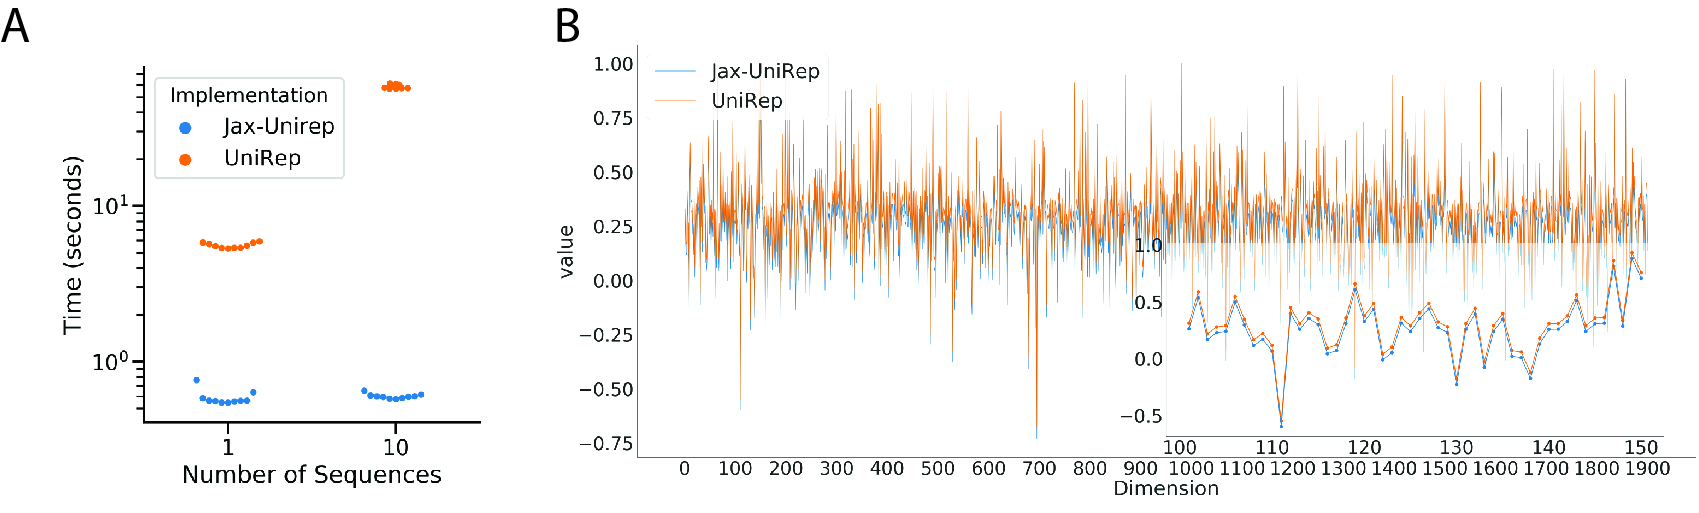
\includegraphics[width=6in]{fig01.jpg}}
    \caption{
        A. Speed comparison between the original implementation (UniRep)
        and our re-implementation (jax-unirep).
        Both one and ten random sequences of length ten
        were transformed by both implementations.
        B. Comparison of the average hidden state between the implementations
        when transforming the same sequence.
        The inset shows a slice of length 50 out of the total 1900 dimensions.
    }
    \label{fig:01}
\end{figure*}

To investigate the performance of \verb|tf-unirep|,
we used Python's \verb|cProfile| facility to identify speed bottlenecks.
On the basis of this, we hypothesized that the cause of speed problems
was graph compilation in TF1.x,
and that we could obtain speedups by using
a non-graph-compiled tensor library.

There were three options available: TF2.x, PyTorch (\cite{pytorch})
and JAX (\cite{jax2018github}).
We chose JAX, because it provides automatic differentiation
on top of the idiomatic NumPy API (\cite{oliphant2006guide}).
Using a familiar API with additional performant primitive functions,
e.g. \verb|lax.scan|, \verb|jit| and \verb|vmap|
reduces the barrier to community contributions.

\section{Software Improvements}

\subsection{Processing multiple protein sequences}

Processing multiple sequences is one place where \verb|jax-unirep|
is more user-friendly than \verb|tf-unirep|.
In \verb|tf-unirep|, to process multiple sequences,
an end-user would call \verb|babbler.get_reps(sequence)| in a loop,
essentially repeatedly paying the TensorFlow graph compilation penalty.
Alternatively, they would have to manually preprocess sequences
into the tensorized embedding using custom code
before passing them into the UniRep model,
impeding reproducibility of model usage results,
and making comparisons between users extremely difficult.

With \verb|jax-unirep|,
to obtain numeric representations of single and multiple protein sequences,
end-users use the high-level function \verb|get_reps()|,
which we have designed to accept single sequences,
multiple sequences of the same length, and
multiple sequences of different lengths.
In each case, tensorized embedding of strings happens automatically,
reducing the chance of user error affecting modelling results,
enforcing consistency between model usage runs.

\subsection{Evolutionary tuning}

"Evotuning" is fine-tuning of the UniRep weights
for a defined collection
of evolutionarily-related protein sequences (\cite{alley2019unified}).
Here, we provide a \verb|fit()| function to perform this task,
in which most of the code necessary for preprocessing the sequences
and performing gradient updates to the weights
are abstracted away from the end-user.
Additionally, automatic checkpointing
into a user-specified directory is available,
allowing users to select
which "evotuned" weights along the optimization path
they wish to use.

\subsection{Software testing and documentation}

We also provide software tests and documentation,
two pieces sorely lacking in \verb|tf-unirep|.
In particular, our test suite covers nearly 90\% of the codebase;
not only are core tensor operations tested for shape correctness,
we have also unit- and integration-tested
the majority of user-facing functions.
As such, end-users can use the model reproducibly with confidence.

\subsection{Speed enhancements}

In a formal speed comparison, we found that \verb|jax-unirep|
performed up to 100X faster on the task of computing protein representations
(using the \verb|get_reps()| function) (Figure 1A\vphantom{\ref{fig:01}}).
We did not test more than 10 sequences
as the original unirep implementation would have taken
an unreasonably long amount of time to run
when using the comparable \verb|babbler.get_reps()| class method.
Comparisons to manual preprocessing for multiple sequences were not done,
as it would not correspond to what we believe to be
the most natural usage pattern of a first-time user of the original model:
simply looping over sequences rather than perform custom preprocessing.
Speed comparisons were performed on a single core of a 24-core
CentOS7 workstation running Intel Xeon processors at 3.6 GHz
with at least 7 replicates.

\section{Reimplementation Verification}

To check that \verb|jax-unirep| was implemented correctly,
we computed numeric representations for single protein sequences
using the original and the reimplementation.
Figure 1B\vphantom{\ref{fig:01}} shows, for one example sequence,
that the representations are identical;
the difference in the traces were injected after computation
merely to visually separate them.

\section{Discussion and Future Work}

Through our reimplementation of UniRep,
we have effectively provided it with non-trivial upgrades over the original.
Having verified its correctness in reimplementation,
we have improved the API, added software tests,
and sped up model forward pass speed by nearly 100X,
all of which are significant upgrades over the original implementation.

Significant effort was invested in accelerating, refactoring, documenting,
and testing the \verb|babbler1900| model.
This was the model with the largest "capacity" by number of parameters),
and likely is the most powerful of the three described in the original paper.
Future work includes implementing
the \verb|babbler256| and \verb|babbler64| models.

\section{Acknowledgements}

We would like to acknowledge the original UniRep authors
for open sourcing their implementation,
our colleagues in the Protein Engineering Platform at NIBR
for providing a use case for the model,
and our beta tester colleagues
in the Chemical Biology and Therapeutics platform at NIBR.

\bibliography{references}
\bibliographystyle{natbib}

\end{document}
